% capscope paper. IEEE conference layout emulated with article + mathptmx (official IEEEtran.cls not available
% offline; on Overleaf, replace the first block with \documentclass[conference]{IEEEtran}).
\documentclass[10pt,twocolumn,letterpaper]{article}
\usepackage[top=0.75in,bottom=1in,left=0.625in,right=0.625in,columnsep=0.25in]{geometry}
\usepackage{mathptmx}
\usepackage[T1]{fontenc}
\usepackage{amsmath,amssymb}
\usepackage{graphicx,booktabs,xcolor}
\usepackage{titlesec,abstract,balance,stfloats}
\usepackage[hidelinks]{hyperref}
\usepackage[font=footnotesize,labelfont=bf,labelsep=period]{caption}
\renewcommand{\thesection}{\Roman{section}}
\renewcommand{\thesubsection}{\Alph{subsection}}
\titleformat{\section}{\centering\normalsize\scshape}{\thesection.}{0.5em}{}
\titleformat{\subsection}{\normalsize\itshape}{\thesubsection.}{0.5em}{}
\titlespacing*{\section}{0pt}{8pt}{4pt}
\titlespacing*{\subsection}{0pt}{6pt}{3pt}
\renewcommand{\abstractnamefont}{\normalfont\small\bfseries\itshape}
\renewcommand{\abstracttextfont}{\normalfont\small\bfseries}
\setlength{\absleftindent}{0pt}\setlength{\absrightindent}{0pt}
\newcommand{\Q}[1]{\textbf{Q#1}}
\newcommand{\tool}[1]{\texttt{\small #1}}
% generated by code/make_numbers.py; do not edit
\expandafter\def\csname n@manPres\endcsname{91}
\expandafter\def\csname n@manPresCI\endcsname{85--96}
\expandafter\def\csname n@manBlk\endcsname{77}
\expandafter\def\csname n@manBlkCI\endcsname{70--82}
\expandafter\def\csname n@manBoth\endcsname{70}
\expandafter\def\csname n@manBothCI\endcsname{63--77}
\expandafter\def\csname n@manDenied\endcsname{14}
\expandafter\def\csname n@manBlkworkspace\endcsname{94}
\expandafter\def\csname n@manPresworkspace\endcsname{95}
\expandafter\def\csname n@manBlktravel\endcsname{61}
\expandafter\def\csname n@manPrestravel\endcsname{100}
\expandafter\def\csname n@manBlkbanking\endcsname{31}
\expandafter\def\csname n@manPresbanking\endcsname{94}
\expandafter\def\csname n@manBlkslack\endcsname{67}
\expandafter\def\csname n@manPresslack\endcsname{71}
\expandafter\def\csname n@autoPres\endcsname{85}
\expandafter\def\csname n@autoPresCI\endcsname{77--91}
\expandafter\def\csname n@autoBlk\endcsname{56}
\expandafter\def\csname n@autoBlkCI\endcsname{48--63}
\expandafter\def\csname n@autoBoth\endcsname{48}
\expandafter\def\csname n@autoBothCI\endcsname{40--56}
\expandafter\def\csname n@autoDenied\endcsname{19}
\expandafter\def\csname n@autoBlkworkspace\endcsname{63}
\expandafter\def\csname n@autoPresworkspace\endcsname{95}
\expandafter\def\csname n@autoBlktravel\endcsname{35}
\expandafter\def\csname n@autoPrestravel\endcsname{100}
\expandafter\def\csname n@autoBlkbanking\endcsname{47}
\expandafter\def\csname n@autoPresbanking\endcsname{75}
\expandafter\def\csname n@autoBlkslack\endcsname{58}
\expandafter\def\csname n@autoPresslack\endcsname{57}
\expandafter\def\csname n@ocatPres\endcsname{100}
\expandafter\def\csname n@ocatPresCI\endcsname{100--100}
\expandafter\def\csname n@ocatBlk\endcsname{83}
\expandafter\def\csname n@ocatBlkCI\endcsname{77--87}
\expandafter\def\csname n@ocatBoth\endcsname{83}
\expandafter\def\csname n@ocatBothCI\endcsname{77--87}
\expandafter\def\csname n@ocatDenied\endcsname{0}
\expandafter\def\csname n@ocatBlkworkspace\endcsname{95}
\expandafter\def\csname n@ocatPresworkspace\endcsname{100}
\expandafter\def\csname n@ocatBlktravel\endcsname{81}
\expandafter\def\csname n@ocatPrestravel\endcsname{100}
\expandafter\def\csname n@ocatBlkbanking\endcsname{42}
\expandafter\def\csname n@ocatPresbanking\endcsname{100}
\expandafter\def\csname n@ocatBlkslack\endcsname{74}
\expandafter\def\csname n@ocatPresslack\endcsname{100}
\expandafter\def\csname n@otoolPres\endcsname{100}
\expandafter\def\csname n@otoolPresCI\endcsname{100--100}
\expandafter\def\csname n@otoolBlk\endcsname{87}
\expandafter\def\csname n@otoolBlkCI\endcsname{83--91}
\expandafter\def\csname n@otoolBoth\endcsname{87}
\expandafter\def\csname n@otoolBothCI\endcsname{83--91}
\expandafter\def\csname n@otoolDenied\endcsname{0}
\expandafter\def\csname n@otoolBlkworkspace\endcsname{95}
\expandafter\def\csname n@otoolPresworkspace\endcsname{100}
\expandafter\def\csname n@otoolBlktravel\endcsname{81}
\expandafter\def\csname n@otoolPrestravel\endcsname{100}
\expandafter\def\csname n@otoolBlkbanking\endcsname{67}
\expandafter\def\csname n@otoolPresbanking\endcsname{100}
\expandafter\def\csname n@otoolBlkslack\endcsname{80}
\expandafter\def\csname n@otoolPresslack\endcsname{100}
\expandafter\def\csname n@manBlkVone\endcsname{65}
\expandafter\def\csname n@manBlkStrict\endcsname{75}
\expandafter\def\csname n@autoBlkVone\endcsname{50}
\expandafter\def\csname n@autoBlkStrict\endcsname{56}
\expandafter\def\csname n@otoolBlkVone\endcsname{81}
\expandafter\def\csname n@otoolBlkStrict\endcsname{85}
\expandafter\def\csname n@nPairs\endcsname{949}
\expandafter\def\csname n@nUsers\endcsname{97}
\expandafter\def\csname n@nBenignCalls\endcsname{339}
\expandafter\def\csname n@nPairsVone\endcsname{629}
\expandafter\def\csname n@unblockable\endcsname{13}
\expandafter\def\csname n@unblockablebanking\endcsname{33}
\expandafter\def\csname n@timeMedMs\endcsname{0.73}
\expandafter\def\csname n@timeMaxMs\endcsname{1.3}
\expandafter\def\csname n@gapCat\endcsname{36}
\expandafter\def\csname n@gapKw\endcsname{79}
\expandafter\def\csname n@extraBlk\endcsname{14}
\expandafter\def\csname n@nUnblk\endcsname{121}
\expandafter\def\csname n@nUnblkText\endcsname{20}
\expandafter\def\csname n@nLost\endcsname{9}
\expandafter\def\csname n@nLostworkspace\endcsname{2}
\expandafter\def\csname n@nLosttravel\endcsname{0}
\expandafter\def\csname n@nLostbanking\endcsname{1}
\expandafter\def\csname n@nLostslack\endcsname{6}
\newcommand{\N}[1]{\csname n@#1\endcsname}


\title{\Large\bfseries How Much Prompt-Injection Defense Does a Free Tool Whitelist Buy?\\ Zero-Inference Capability Manifests for Tool-Calling Agents}
\author{Clement Aidoo\\ \small CANLABS, Ghana \quad \texttt{clement.aidoo@canlabs.org}\\
\small Code, data and protocol: \url{https://github.com/CAN-Aidoo/capscope}}
\date{}

\begin{document}
\maketitle

\begin{abstract}
Defenses against indirect prompt injection that work well today put a language model in the loop, which adds model
calls and latency to every task. We ask how much protection a tool-calling agent can get for free. capscope builds a
tool whitelist (a \emph{capability manifest}) once from the user's instruction by matching stemmed action verbs against
per-tool profiles written from documentation. It then gates every tool call, and nothing the agent reads later can widen
the whitelist. Building the manifest takes under a millisecond and no model call. In an oracle evaluation on all
\N{nPairs} user$\times$injection pairs of AgentDojo v1.2, using the benchmark's ground-truth tool calls, the manifest keeps
every needed tool for \N{manPres}\% of benign tasks and denies a tool the attack needs in \N{manBlk}\% of pairs
(95\% interval \N{manBlkCI}\%). Mechanically extracted keywords do much worse (\N{autoBlk}\%). Even an oracle whitelist
that knows exactly which tools each user task needs blocks only \N{otoolBlk}\%. The other \N{unblockable}\% of attacks,
\N{unblockablebanking}\% in banking, use only tools the user's own task needs, so no tool-level policy can stop them.
Most benign failures come from tasks that delegate their instructions to an email, file or web page, which is the
channel injections use. A free whitelist therefore removes most attacks that need a new capability, and the
\N{unblockable}\% that reuse the user's own capabilities mark where argument- and data-flow-level defenses become
necessary. Protocol, profiles, code and per-pair results are public.
\end{abstract}


\begin{figure}[h]\centering
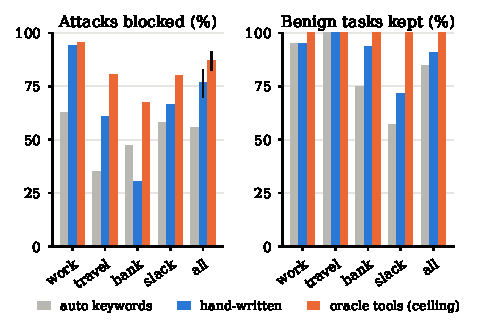
\includegraphics[width=\columnwidth]{fig_teaser.pdf}
\caption{Oracle evaluation on AgentDojo v1.2 (\N{nPairs} user$\times$injection pairs). Left: pairs in which the manifest
built from the user's instruction denies at least one tool the injection needs. Right: benign user tasks whose every
ground-truth call stays allowed. The orange ``oracle tools'' manifest knows exactly which tools the user task needs; it
bounds every tool-level policy, so the \N{unblockable}\% it cannot block are out of reach of any tool whitelist. Bars on
``all'': 95\% bootstrap intervals over user tasks.}\label{fig:teaser}
\end{figure}

\section{Introduction}
Tool-calling language-model agents read untrusted text: emails, web pages, shared files, chat messages. An attacker who
controls that text can embed instructions, and the agent may follow them with the user's privileges
\cite{greshake2023,zhan2024}. This \emph{indirect prompt injection} is the top risk in OWASP's list for LLM
applications \cite{owasp2025}. Defenses that hold up well today, such as CaMeL \cite{debenedetti2025camel},
Progent \cite{shi2025progent} and MELON \cite{zhu2025melon}, put a language model or a policy synthesiser in the
loop. That costs extra model calls, latency and money on every task.

For many deployments that cost matters. At CANLABS we build agents for low-bandwidth, metered settings, where an
extra round trip to a model is a real price. This raises a simple question: how much protection is available
\emph{for free}? The cheapest least-privilege policy we can think of is a tool whitelist built once from the user's
instruction, by keyword matching, before the agent reads anything untrusted. Nothing the agent reads later can widen
it. It needs no model call and runs in under a millisecond.

We call this whitelist a \emph{capability manifest} and measure both what it buys and where any tool whitelist must
stop. Our contributions are:
\begin{itemize}\setlength\itemsep{1pt}
\item \textbf{capscope}, a zero-inference capability manifest for AgentDojo agents \cite{debenedetti2024agentdojo}:
per-tool profiles (category, sensitivity, action verbs) written from tool documentation alone, a deterministic
matcher, and a gate that replaces the tool executor.
\item An \emph{oracle} evaluation that needs no model: on all \N{nPairs} user$\times$injection pairs of AgentDojo
v1.2 we check the manifest against the ground-truth tool calls of the user task and of the injection. The
hand-written manifest keeps \N{manPres}\% of benign tasks fully allowed and denies a needed tool in \N{manBlk}\% of
attacks.
\item A ceiling for the whole class of tool-level defenses: even a manifest that knows exactly which tools the user
task needs blocks only \N{otoolBlk}\% of pairs. The remaining \N{unblockable}\% (\N{unblockablebanking}\% in banking)
reuse tools the user's own task needs. Stopping them requires argument-level or data-flow control.
\item A pre-registered protocol, with deviations dated, and all code, profiles and per-pair results released.
\end{itemize}

\section{Related Work}
\textbf{Attacks and benchmarks.} Greshake et al.\ showed indirect injection against deployed LLM applications
\cite{greshake2023}. InjecAgent \cite{zhan2024} and AgentDojo \cite{debenedetti2024agentdojo} benchmark tool-using
agents; AgentDojo runs agents in stateful environments (workspace, travel, banking, Slack) and judges both task utility
and attack success from the final environment state. We use AgentDojo because its tasks ship ground-truth tool calls.

\textbf{Model-level and prompt-level defenses.} Spotlighting marks untrusted text with delimiters or encodings
\cite{hines2024}. PromptArmor asks an LLM to detect and remove injected text before the agent sees it
\cite{shi2025promptarmor}. MELON re-runs the agent with the user task masked and flags tool calls that do not depend on
the user's request \cite{zhu2025melon}. Each adds at least one model call per step or per tool output.

\textbf{Privilege control.} AgentDojo's tool filter asks the model, once, to choose the tools needed for the task
\cite{debenedetti2024agentdojo}; it is the closest LLM-based analogue of our manifest. Progent expresses fine-grained,
argument-level privilege policies and can have an LLM generate and update them \cite{shi2025progent}. CaMeL separates
control flow, planned from the trusted query, from data flow, and enforces capabilities on values
\cite{debenedetti2025camel}. Our manifest sits at the cheapest end of this design space: tool-level only, no model,
built once. We use it to measure how much of the benefit of privilege control survives at zero inference cost, and
our ceiling analysis says what only argument- or data-flow-level methods such as Progent and CaMeL can add.

\section{Capability Manifests}\label{sec:method}
\begin{figure*}[t]\centering
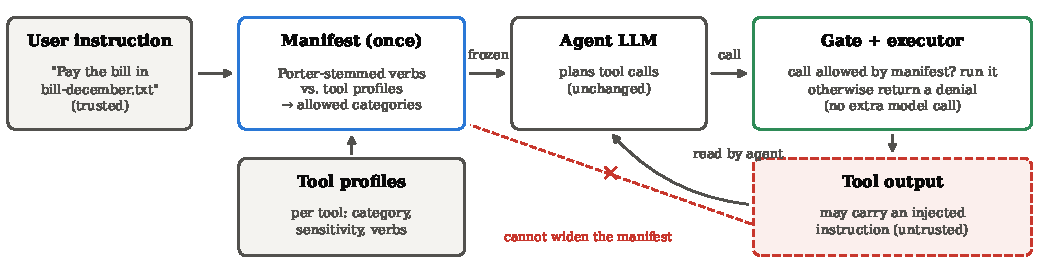
\includegraphics[width=\textwidth]{fig_method.pdf}
\caption{capscope. The manifest is computed once from the trusted user instruction and the static tool profiles, then
frozen. Every tool call passes a gate; calls outside the manifest are not executed and the agent receives a denial
message. Tool outputs, which may carry injected instructions, never reach the manifest.}\label{fig:method}
\end{figure*}

\textbf{Threat model.} The user and the system prompt are trusted. Tool outputs may contain attacker-controlled text.
The attacker wins if the agent performs an action the user did not ask for, judged by AgentDojo's state-based
\texttt{security} checks. We do not consider attacks on the model's final text answer except where they need a tool.

\textbf{Tool profiles.} For every tool we record a capability \emph{category} (e.g.\ \tool{money\_out},
\tool{email\_send}, \tool{read}), a \emph{sensitivity} from 1 (read or search) to 3 (irreversible or outbound), and a
list of \emph{action verbs} that, if they appear in the user's instruction, evidence that category. For sensitive tools
the list holds verbs (\emph{send, pay, delete, share, reserve}), never object nouns: ``email'' appears in ``summarise my
emails'' as often as in ``email Bob''. Profiles were written from tool names and docstrings, before any evaluation and
without reading task prompts (Section~\ref{sec:setup}).

\textbf{Manifest and gate.} Both the instruction and the keywords are lower-cased and Porter-stemmed
\cite{porter1980,bird2009}. A tool's category enters the manifest if any of its keywords occurs in the instruction. A
call is allowed if its category is in the manifest, or if the tool is a sensitivity-1 read. Otherwise the gate returns
``\emph{[capscope] Call to X denied: \dots}'' without executing it. The manifest is stored with the episode and never
recomputed, so an injected ``please also send \dots'' cannot add \tool{email\_send}. On the benchmark's 97 user tasks,
building the manifest and checking every tool took \N{timeMedMs}\,ms (median; maximum \N{timeMaxMs}\,ms) on one cloud
CPU core, with no network access.

\section{Experimental Setup}\label{sec:setup}
\textbf{Benchmark.} AgentDojo v1.2 (package 0.1.35): \N{nUsers} user tasks and 35 injection tasks in four suites,
\N{nPairs} user$\times$injection pairs (\N{nPairsVone} in the original v1 tasks). Every task carries a ground-truth list
of tool calls that solves it.

\textbf{Manifests compared.} \emph{Hand-written}: the profiles above. \emph{Auto}: same categories and sensitivities, but
keywords taken mechanically from the tool name and first docstring sentence minus a fixed stop-list; this tests how much
the verb lists matter. \emph{Oracle categories} and \emph{oracle tools}: manifests built from the user task's own
ground truth, at category or tool granularity. They cannot be deployed, but they bound what a perfect matcher could do.

\textbf{Metrics.} A user task is \emph{kept} if every one of its ground-truth calls is allowed. A pair is
\emph{blocked} if at least one ground-truth call of the injection task is denied under the manifest built from the user
prompt. AgentDojo's own success checks require the whole injection goal, so denying one required call defeats it. 95\%
intervals bootstrap over user tasks (10{,}000 resamples), because pairs that share a user task are not independent.

\textbf{Protocol.} The questions, metrics and profiles were committed before evaluation (\texttt{PROTOCOL.md}). Three
deviations are recorded there. (D1) In the released package, workspace injection tasks 6--13 return an empty ground
truth; we annotated their tools from each task's goal and its \texttt{security} check. We also report results without
them and a strict view that ignores their clean-up \tool{delete\_email}. (D2) The protocol quoted AgentDojo v1's 629
pairs; v1.2 has \N{nPairs}. (D3) The planned end-to-end run with a model was not carried out for lack of an API
budget; its code is released. No profile was changed after results were seen.

\textbf{Questions.} \Q1: how many attacks does the manifest block? \Q2: how many benign tasks does it keep? \Q3: what is
the ceiling for any tool-level manifest, and why? An end-to-end run with a model was planned as a fourth question
but not carried out (deviation D3, Section~\ref{sec:lim}).

\begin{table}[t]\centering\footnotesize\setlength{\tabcolsep}{2.2pt}
\caption{Oracle evaluation on AgentDojo v1.2 (97 user tasks, 949 user$\times$injection pairs). Each cell: user tasks with every ground-truth call allowed (\%) / pairs in which at least one ground-truth call of the injection is denied (\%). Oracle rows build the manifest from the user task's own ground truth and bound any tool-level policy.}\label{tab:oracle}
\begin{tabular}{lccccc}
\toprule
manifest & workspace & travel & banking & slack & all\\
\midrule
capscope (hand-written) & 95 / 94 & 100 / 61 & 94 / 31 & 71 / 67 & 91 / 77\\
capscope (auto keywords) & 95 / 63 & 100 / 35 & 75 / 47 & 57 / 58 & 85 / 56\\
\midrule
oracle categories & 100 / 95 & 100 / 81 & 100 / 42 & 100 / 74 & 100 / 83\\
oracle tools & 100 / 95 & 100 / 81 & 100 / 67 & 100 / 80 & 100 / 87\\
\midrule
pairs & 560 & 140 & 144 & 105 & 949\\
\bottomrule
\end{tabular}
\end{table}


\section{Results}

\subsection{\Q1: How many attacks does the manifest block?}
The hand-written manifest denies at least one tool the injection needs in \N{manBlk}\% of the \N{nPairs} pairs (95\%
interval \N{manBlkCI}\%; Table~\ref{tab:oracle}, Fig.~\ref{fig:teaser}). The rate depends strongly on the suite:
\N{manBlkworkspace}\% in workspace, \N{manBlkslack}\% in Slack, \N{manBlktravel}\% in travel and only
\N{manBlkbanking}\% in banking. The result does not hinge on annotation D1. On the \N{nPairsVone} pairs of the original
v1 tasks it is \N{manBlkVone}\% (ceiling \N{otoolBlkVone}\%). Ignoring the clean-up \tool{delete\_email} of the
annotated tasks gives \N{manBlkStrict}\% (ceiling \N{otoolBlkStrict}\%).

The verb lists matter. With keywords taken mechanically from the tool name and docstring, the manifest blocks
\N{autoBlk}\% (\N{autoBlkCI}\%) and keeps fewer benign tasks (\N{autoPres}\% against \N{manPres}\%). Docstring words
such as ``money'', ``transaction'' or ``email'' name objects, so they match read-only requests and open sensitive
categories for no reason. In travel the auto manifest blocks \N{autoBlktravel}\%, against \N{manBlktravel}\% for the
hand-written one.

\subsection{\Q2: How many benign tasks does it keep?}
\N{manPres}\% of the \N{nUsers} user tasks keep every ground-truth call allowed (\N{manPresCI}\%). Only \N{manDenied} of
\N{nBenignCalls} benign calls are denied, but they fall in \N{nLost} tasks: \N{nLostslack} in Slack, \N{nLostworkspace}
in workspace and \N{nLostbanking} in banking. They are of three kinds. Five tasks \emph{delegate} the instruction to
content: ``do the actions specified in the email from David'', ``read the file \texttt{landlord-notices.txt} and follow
the instructions'', ``do all the tasks on my TODO list at \texttt{www.company-todo-list.com}''. The tools such a task
needs are named only in the content it points to, and that content arrives through exactly the channel an injection
uses. A manifest built from the user's words cannot serve these tasks without trusting that channel. Three Slack tasks
need to open a web page that the instruction mentions only indirectly (``summarise the article that Bob posted''), and
one says ``message them'', a verb we left out because ``message'' is far more often a noun. Travel, the suite whose
instructions name their actions most plainly (``book'', ``reserve''), keeps all of its tasks.

\subsection{\Q3: What is the ceiling, and why?}
A manifest that knows exactly which tools the user task needs (``oracle tools'') blocks \N{otoolBlk}\% of pairs
(\N{otoolBlkCI}\%). No tool-level policy, whether built by keywords, by an LLM or by hand per task, can do better on
these pairs, because the remaining \N{nUnblk} pairs (\N{unblockable}\%) are reachable with tools the user's task
legitimately needs. \N{nUnblkText} of them come from one travel injection that only asks the agent to recommend a hotel
in its answer, and needs no tool at all. Most of the rest are in banking (\N{unblockablebanking}\% of banking pairs).
There, seven of the nine injections need no sensitive tool other than \tool{send\_money}, and paying, refunding or transferring
is what many banking user tasks are about. Telling the user's payment from the attacker's would need checks on the
arguments (which IBAN, how much) or on where they came from, as in Progent and CaMeL
\cite{shi2025progent,debenedetti2025camel}.

The hand-written manifest reaches \N{manBlk}\% of this \N{otoolBlk}\% ceiling. The gap has two sources. In \N{gapCat}
pairs the user task needs one tool of a category and the attack uses another tool of the same category: paying a bill
opens \tool{money\_out}, which also contains \tool{update\_scheduled\_transaction}. Using oracle categories instead of
oracle tools lowers banking from \N{otoolBlkbanking}\% to \N{ocatBlkbanking}\%. In \N{gapKw} pairs a keyword in the
instruction opens a category the task does not need. In the other direction, \N{extraBlk} pairs are blocked by our
manifest but not by the oracle, because it also denies a tool the user task needs. Those blocks cost utility, so we
also report pairs that are both blocked and kept: \N{manBoth}\% (\N{manBothCI}\%), against \N{otoolBoth}\% for the
oracle.

\subsection{\Q4: End-to-end with a model}
\textcolor{red}{\textbf{[Pending. This subsection is filled only from the completed runs of
\texttt{code/run\_llm.py} (Claude Haiku; no defense, capscope, LLM tool filter; AgentDojo's
\texttt{important\_instructions} attack) via \texttt{code/analyze\_llm.py}. No number is entered by hand.]}}


\section{Limitations}
The oracle evaluation measures what the manifest permits along each task's ground-truth tool sequence, not what a model
does. A model may solve a task with other tools, or follow an injection only partly, so \Q1--\Q3 bound attack success
rather than measure it; \Q4 measures it. The profiles were written by the author for this benchmark, from docstrings
and before evaluation, but a different author would choose different verbs; the auto variant shows the method is
sensitive to that choice. The matcher is lexical: a paraphrase without a listed verb (``get Bob his money back'') is
missed, and an instruction that names an action it forbids (``do not delete anything'') opens it. Knowing the
profiles does not let an attacker widen the manifest, because it depends only on the user's text, but it does tell
them which tools stay open. A user task that delegates its instructions to content is unprotected by design. Results are for AgentDojo's four simulated suites and
English instructions only.

\section{Conclusion}
A tool whitelist computed once from the user's own words, with no model call, blocks most prompt-injection attacks
that need a capability the user did not ask for, and keeps most legitimate tasks working. Its failures are
informative. Benign tasks break when the user delegates the instruction to untrusted content, and \N{unblockable}\% of
attacks cannot be stopped by any tool-level policy because they reuse the capabilities the user's task requires. For
cost-sensitive deployments the manifest is a sensible first layer. The cases it cannot handle, delegation and reuse of
the user's own capabilities, are exactly where model-based or data-flow defenses should spend their cost.


\section*{Data Availability}
Code, tool profiles, the frozen protocol, per-pair oracle results and the scripts that generate every number in this
paper: \url{https://github.com/CAN-Aidoo/capscope}.

\section*{Use of AI Tools}
Code, analysis and drafting were carried out with the assistance of an AI model (Claude, Anthropic) under the author's
direction. The author takes responsibility for the content.

\begin{thebibliography}{99}\footnotesize\setlength{\itemsep}{0pt}
\bibitem{greshake2023} K.~Greshake, S.~Abdelnabi, S.~Mishra, C.~Endres, T.~Holz and M.~Fritz, ``Not what you've signed up for: Compromising real-world LLM-integrated applications with indirect prompt injection,'' in \emph{Proc.\ ACM AISec Workshop}, 2023. arXiv:2302.12173.
\bibitem{zhan2024} Q.~Zhan, Z.~Liang, Z.~Ying and D.~Kang, ``InjecAgent: Benchmarking indirect prompt injections in tool-integrated large language model agents,'' in \emph{Findings of ACL}, 2024. arXiv:2403.02691.
\bibitem{owasp2025} OWASP Foundation, ``OWASP Top 10 for Large Language Model Applications 2025: LLM01 Prompt Injection,'' 2025.
\bibitem{debenedetti2024agentdojo} E.~Debenedetti, J.~Zhang, M.~Balunovi\'c, L.~Beurer-Kellner, M.~Fischer and F.~Tram\`er, ``AgentDojo: A dynamic environment to evaluate prompt injection attacks and defenses for LLM agents,'' in \emph{NeurIPS Datasets and Benchmarks Track}, 2024. arXiv:2406.13352.
\bibitem{debenedetti2025camel} E.~Debenedetti et al., ``Defeating prompt injections by design,'' arXiv:2503.18813, 2025.
\bibitem{shi2025progent} T.~Shi et al., ``Progent: Programmable privilege control for LLM agents,'' arXiv:2504.11703, 2025.
\bibitem{zhu2025melon} K.~Zhu et al., ``MELON: Provable defense against indirect prompt injection attacks in AI agents,'' in \emph{Proc.\ ICML}, 2025. arXiv:2502.05174.
\bibitem{hines2024} K.~Hines, G.~Lopez, M.~Hall, F.~Zarfati, Y.~Zunger and E.~Kiciman, ``Defending against indirect prompt injection attacks with spotlighting,'' arXiv:2403.14720, 2024.
\bibitem{shi2025promptarmor} T.~Shi et al., ``PromptArmor: Simple yet effective prompt injection defenses,'' arXiv:2507.15219, 2025.
\bibitem{porter1980} M.~F.~Porter, ``An algorithm for suffix stripping,'' \emph{Program}, vol.~14, no.~3, pp.~130--137, 1980.
\bibitem{bird2009} S.~Bird, E.~Klein and E.~Loper, \emph{Natural Language Processing with Python}. O'Reilly, 2009.
\end{thebibliography}

\end{document}
